% Dokumenteinstellungen
% ======================================================================

% Dokumentklasse (Schriftgröße 6, DIN A4, Artikel)
\documentclass[9pt,a4paper]{scrartcl}


% Pakete laden
\usepackage[utf8]{inputenc}		% Zeichenkodierung: UTF-8 (für Umlaute)   
\usepackage[german]{babel}		% Deutsche Sprache
\usepackage{amsmath}			% erlaubt mathematische Formeln
\usepackage{amssymb}			% Verschiedene Symbole
\usepackage{esint}				% erweiterte Integralsymbole
\usepackage{multicol}			% ermöglicht Seitenspalten  
\usepackage{booktabs}			% bessere Tabellenlinien
\usepackage{graphicx}			% Zum Bilder einfügen benötigt
\usepackage{pbox}				%Intelligent parbox: \pbox{maximum width}{blabalbalb \\ blabal}
\usepackage{accents}			% Für eigene Ableitungspunkte benötigt
\usepackage{scrtime}
\usepackage{titlesec}


% .:: Seitenlayout und Ränder
% ======================================================================
\usepackage{geometry}
\geometry{a4paper,landscape, left=5mm,right=20mm, top=6mm, bottom=5mm, includefoot} 
	
% Schriftart SANS für bessere Lesbarkeit bei kleiner Schrift
\renewcommand{\familydefault}{\sfdefault} 
% Array- und Tabellenabstände vergrößern
\renewcommand{\arraystretch}{1.2}

% Eigene Befehle
\newcommand{\iset}[2]{\ensuremath{\bigl\{ \bigl. #1 \, \bigr| \, #2 \bigr\}}}	%intensional set
\newcommand{\eset}[1]{\ensuremath{\bigl\{#1\bigr\}}}							%extensional set
\newcommand{\enbrace}[1]{\ensuremath{\bigl\(#1\bigr\)}}							%große Klammern
\newcommand{\norm}[1]{\ensuremath{\|#1\|}}										%Norm
\newcommand{\abs}[1]{\ensuremath{\left\vert#1\right\vert}} 						%Betrag
\newcommand{\mat}[1]{\ensuremath{\begin{bmatrix} #1 \end{bmatrix}}}				%Matrix
\newcommand{\ma}[1]{\ensuremath{\utilde{\boldsymbol {#1}}}}						%Matrixsymbol
\newcommand{\vect}[1]{\ensuremath{\begin{pmatrix} #1 \end{pmatrix}}}			%Vektor
\newcommand{\mvect}[1]{\ensuremath{\left. \begin{matrix} #1 \end{matrix}  \right]}} %Matrixvektor
\newcommand{\gk}[1]{\ensuremath{\left\lfloor#1\right\rfloor}} 					%Gaußklammer
\newcommand{\sprod}[2]{\ensuremath{\left\langle #1, #2 \right\rangle }}			%Skalarprodukt
\newcommand{\bdot}{\ensuremath{\boldsymbol \cdot}} 								%Dicker Punkt für Skalarprodukt


% Befehle sichern
\let\oldvec = \vec
\let\olddot = \dot

% Überschreibungen
\renewcommand{\vec}[1]{\ensuremath{\underline{\boldsymbol {#1}}}}
\renewcommand{\emph}[1]{\textbf{#1}}
\renewcommand*{\dot}[1]{\accentset{\mbox{\textrm{\large\bfseries .}} }{#1}}
\renewcommand*{\ddot}[1]{\accentset{\mbox{\textrm{\large\bfseries .\hspace{-0.25ex}.}}}{#1}}
\renewcommand{\i}{\ensuremath{\mathrm{j}}}										%imaginäre Einheit

% Abkürzungen
\newcommand{\ul}[1]{\ensuremath{\underline{#1}}}								%Untersteichen
\newcommand{\ol}[1]{\ensuremath{\overline{#1}}}									%Überstreichen
\newcommand{\Ra}[0]{\ensuremath{\Rightarrow}}									%Rightarrow
\newcommand{\ra}[0]{\ensuremath{\rightarrow}} 									%Rightarrow
\newcommand{\bs}[1]{\ensuremath{\boldsymbol{#1}}}								%Fett und kursiv im mathmode
\newcommand{\diff}{\ensuremath{\ \mathrm d}}									%delta
\newcommand{\grad}{\ensuremath{\mathrm{grad}\,}}								%Gradient
\renewcommand{\div}{\ensuremath{\mathrm{div}\,}}								%Divergenz
\newcommand{\rot}{\ensuremath{\mathrm{rot}\,}}									%Rotation
\newcommand{\Sp}{\ensuremath{\mathrm{Sp}\,}}									%Spur
\newcommand{\ggT}{\ensuremath{\mathrm{ggT\,}}}									%ggT
\newcommand{\e}{e}																%Eulersche Zahl
	% Für Mengen
	\newcommand{\N}{\ensuremath{\mathbb N}}
	\newcommand{\R}{\ensuremath{\mathbb R}}
	\newcommand{\C}{\ensuremath{\mathbb C}}
	\newcommand{\Z}{\ensuremath{\mathbb Z}}
	\newcommand{\K}{\ensuremath{\mathbb K}}


% .:: Kopf- und Fußzeile
% ======================================================================
\usepackage{fancyhdr}
\pagestyle{fancy}
\fancyhf{}

	\fancyfoot[C]{\small von Benedikt Schmidt}
   \renewcommand{\headrulewidth}{0.0pt} %obere Linie ausblenden
   \renewcommand{\footrulewidth}{0.1pt} %obere Linie ausblenden

   \fancyfoot[R]{\small Stand: \today \ um \thistime \ Uhr \qquad \thepage}
   \fancyfoot[L]{\small Homepage: www.latex4ei.de -- Fehler bitte \emph{sofort} melden.}



	
% Formatierung der Überschriften
\titleformat{\section}{\huge \bfseries}{\thesection}{1em}{}
\titleformat{\subsection}{\bfseries}{\thesubsection}{1em}{}


% Dokumentbeginn
% ======================================================================
\begin{document}


% Aufteilung in Spalten
\begin{multicols}{3}

% ---------------------------------------
% | 		Energietechnik	 			|
% ~~~~~~~~~~~~~~~~~~~~~~~~~~~~~~~~~~~~~~~
%=======================================================================

	\section{Allgemeines}
		\subsection{Mathematische Grundlagen}
		Cramersche Regel: $A x = b$; $A_i$ ist i-te Spalte durch b ersetzt
		\[x_i = \frac{det(A_i)}{det(A)}\]	
		\[Z = R + j X \Rightarrow X = \frac{Z}{\sqrt{1 + \left( \frac{R}{X}\right)^2}}\]

		\subsection{Physikalische Grundlagen}
		\[P = F \cdot v = M \cdot \omega\]
		\[\omega = \frac{\diff \varphi}{\diff t} = 2 \pi n = 2 \pi f = \frac{v}{r}\]

		\subsection{Lastganglinien}
		$T_n$: Nennbetriebsdauer\\
		$T_a$ Ausnutzungsadauer\\
		$T_{ben}$: Benutzungsdauer\\
		$P_{max}$: Höchstlast\\
		\[W = P_{mittel} T_n = P_n T_a = P_{max} T_{ben}\]
		
		\subsection{Netzumformungen - Dreieck-Stern}
		\[\vec Z_{12} = \frac{\vec Z_1 \vec Z_2 + \vec Z_2 \vec Z_3 + \vec Z_3 \vec Z_1}{\vec Z_3}\]
		\[\vec Z_{23} = \frac{\vec Z_1 \vec Z_2 + \vec Z_2 \vec Z_3 + \vec Z_3 \vec Z_1}{\vec Z_1}\]
		\[\vec Z_{31} = \frac{\vec Z_1 \vec Z_2 + \vec Z_2 \vec Z_3 + \vec Z_3 \vec Z_1}{\vec Z_2}\]
		
		\[\vec Z_1 = \frac{\vec Z_{12} \vec Z_{31}}{\vec Z_{12} + \vec Z_{23} + \vec Z_{31}}\]
		\[\vec Z_2 = \frac{\vec Z_{12} \vec Z_{23}}{\vec Z_{12} + \vec Z_{23} + \vec Z_{31}}\]
		\[\vec Z_3 = \frac{\vec Z_{23} \vec Z_{31}}{\vec Z_{12} + \vec Z_{23} + \vec Z_{31}}\]
	
	\section{Wechel-/Drehstromsystem}
		\subsection{Wechselstromsystem}
		\[\varphi = \varphi_u - \varphi_i\]		
		\[u(t) = \hat u \cos(\omega t + \varphi_u) = U \sqrt{2} \cos(\omega t + \varphi_u)\]
		\[i(t) = \hat i \cos(\omega t + \varphi_i) = I \sqrt{2} \cos(\omega t + \varphi_i)\]
		\[\vec u(t) = \hat u \exp\big(\i (\omega t + \varphi_u)\big)\] 
		\[u(t) = \Re(\vec u(t))\]
		\[U = \sqrt{\frac{1}{T} \int_{t_0}^{t_0 + T} u^2(\tau) \diff \tau}\]
	
		\subsection{Komplexe Leistung}
		\[\lambda = \frac{|P|}{S} = \cos(\varphi)\]
		\[p(t) = P + S \cdot \cos(2\omega t + \varphi_u + \varphi_i)\]
		\[\vec S = \vec U \cdot \vec I^\star\]
		\[\tilde {\vec S} = \vec U \cdot \vec I\]

		\subsection{Drehstromsystem}
		\[\vec a = \exp \left(\i \frac{2}{3} \pi \right)\] 
		\[\vec a^0 = \vec a^3 = 1\] 
		\[\vec a^* = \vec a^2\]		
		\[\vec S = \sqrt{3} \cdot \vec U \cdot \vec I^\star\]
		\[\vec S = \vec U_1 \cdot \vec I_1^\star + \vec U_2 \cdot \vec I_2^\star + \vec U_3 \cdot \vec I_3^\star\]
		\[\tilde{\vec S} = \vec U_1 \cdot \vec I_1 + \vec U_2 \cdot \vec I_2 + \vec U_3 \cdot \vec I_3\]
		\[p(t) = \operatorname{Re} \left\{ \vec S \right\} + \operatorname{Re} \left\{\tilde{\vec S} e^{j 2 \omega t} \right\}\]
		
		\subsection{Symmetrische Komponenten}
		(0): Nullsystem; (1): Mitsystem; (2): Gegensystem
		\[\begin{pmatrix} \vec I_{(1)} \\ \vec I_{(2)} \\ \vec I_{(0)} \end{pmatrix} = \frac{1}{3}
		\begin{pmatrix} 1 & \vec a & \vec a^2 \\ 1 & \vec a^2 & \vec a \\ 1 & 1 & 1 \end{pmatrix} 
		\begin{pmatrix} \vec I_1 \\ \vec I_2 \\ \vec I_3 \end{pmatrix}\]
		\[\begin{pmatrix} \vec I_1 \\ \vec I_2 \\ \vec I_3 \end{pmatrix} = 
		\begin{pmatrix} 1 & 1 & 1 \\ \vec a^2 & \vec a & 1 \\ \vec a & \vec a^2 & 1 \end{pmatrix} 
		\begin{pmatrix} \vec I_{(1)} \\ \vec I_{(2)} \\ \vec I_{(0)} \end{pmatrix}\]


	\section{Elektrische Maschinen}
		\subsection{Der Transformator}		
		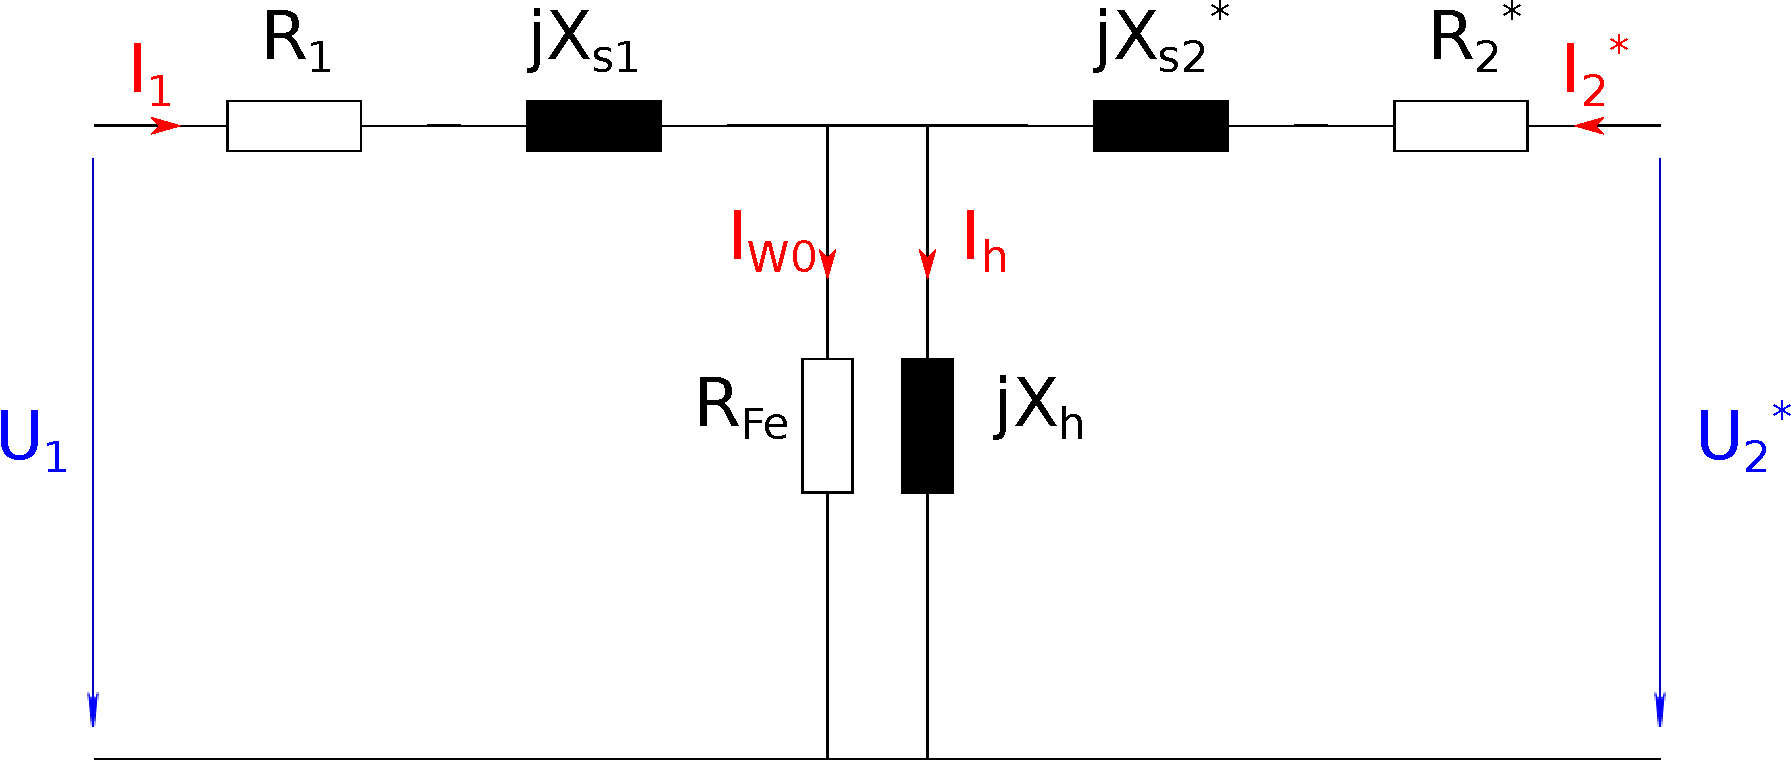
\includegraphics[scale=.3]{./img/ersatzschaltbild_transformator.pdf} \\

		\begin{tabular}{cl}
		ü & Übersetzung \\
		$"u_r$ & Bemessungsübersetzung \\
		$U_{r1T}$, $U_{r2T}$ & Bemessungsspannungen \\
		$S_{rT}$ & Bemessungsleistung \\
		$U_{K}$ & Kurzschlussspannung \\
		$u_k$ & bezogene Kurzschlussspannung \\
		$u_r$ & bezogener Wirkspannungsabfall \\
		$P_{Cu}$ & Kupferverluste \\
		$P_{Fe}$ & Eisenverluste \\
		$Z_k$ & Kurzschlussimpedanz
		\end{tabular}

		\[\vec U^b = "u \vec U\]
		\[\vec I^b = \frac{1}{"u} \vec I\]
		\[\vec Z^b = "u^2 \vec Z\]
		\["u = \frac{W_1}{W_2}\]
		\["u_r = \frac{U_{r1T}}{U_{r2T}}\]
		\[u_k = \frac{U_{K}}{U_{r1T}}\]
		\[Z_k = \frac{U_{kT}}{\sqrt{3}\cdot I_r} = u_k \frac{U_{r1T}^2}{S_{rT}}\]
		\[u_r = \frac{U_{rT}}{U_{r1T}}\]
		\[R_k = P_{Cu} \left( \frac{U_{r1T}}{S_{rT}} \right)^2\]
		\[R_k = u_r \frac{U_{r1T}^2}{S_{rT}}\]
		\[Z_k = \sqrt{R_k^2 + X_k^2}\]
		\[R_{Fe} = \frac{U_{r1T}^2}{P_{Fe}}\]
		\[I_{W0} = \frac{P_{Fe}}{\sqrt{3} U_{r1T}}\]
		\[I_h = \sqrt{I_{10}^2 - I_{W0}^2}\]
		\[X_h = \frac{U_{r1T}}{\sqrt{3} I_h}\]
		
		Parallelbetrieb von Transformatoren:
		\[\frac{S_{T1}}{S_{T2}} = \frac{u_{kT2} \cdot S_{rT1}}{u_{kT1} \cdot S_{rT2}}\]
	
		\subsection{Gleichstrommaschine}
		
		\begin{tabular}{cl}
		$p$ & Polpaarzahl \\
		$z$ & Anzahl der Schaltstufen \\
		$\lambda$ & Schaltverhältnis \\
		$U$ & Ankerklemmenspannung \\
		$U_i$ & Im Anker induzierte Spannung \\
		$K_1$, $K_2$ & Maschinenkonstanten \\
		$\Phi$ & magnetischer Fluss durch den Anker \\
		$I_A$ & Ankerstrom \\
		$R_A$ & Widerstand der Ankerwicklungen \\
		$I_E$ & Erregerstrom
		\end{tabular}
		
		\subsubsection{Grundgleichungen}
		\[U_A = U_i + (R_A + R_v) I_A = U_i + RI\]
		\[U_i = K_1 \Phi n\]
		\[M = K_2 \Phi I_A\]
		\[\Phi = f(I_E)\]
		falls verlustfrei: $K_1 = 2 \pi K_2$ \\
		falls im linearen Bereich: $\Phi = K_3 I_E$ \\
		
		\begin{center}
		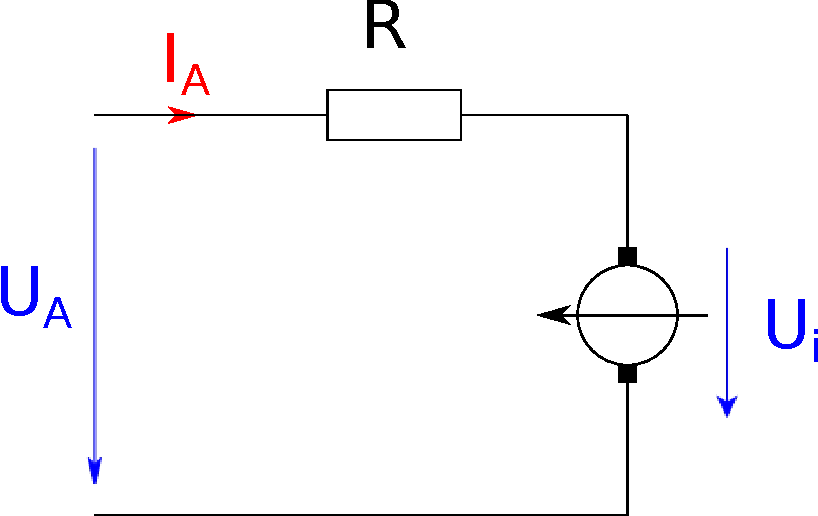
\includegraphics[scale=.4]{./img/ersatzschaltbild_gleichstrommaschine.pdf}
		\end{center}
		
		\subsubsection{Anlaufen mit Vorwiderständen}
		$R_{A_,z-1} = R_A + R_{V1}$, $R_{A_,z-1} = R_A + R_{V1} + R_{V2}$, ..., $R_{A,0} = R_A + R_{V1} + \hdots + R_{Vz}$ \\
		\[\lambda = \frac{M_{max}}{M_{min}} = \frac{R_{A,Z-1}}{R_{A,Z}}\]
		\[z = \log_\lambda \frac{R_{A0}}{R_A}\]
		
		% Bild der Vorwiderstände
		
		\subsubsection{Fremderregt}
		\[n = \frac{U}{ K_1 \cdot \Phi} - \frac{R}{K_1 \cdot K_2 \cdot \phi^2}M\]
		\[n_0 = \frac{U}{K_1 \Phi}\]
		\[M_A = \frac{U K_2 \Phi}{R}\]
		\[n = n_0 - n_0 \frac{M}{M_A}\]
		
		% Ersatzschaltbild
		
		\subsubsection{Reihenschluss}
		\[M = \frac{K_2}{K_3} \Phi^2\]
		\[n = \frac{U}{\sqrt{2 \pi K_1 K_3}} \frac{1}{\sqrt{M}} - \frac{R}{K_1 K_3}\]
		
		% Ersatzschaltbild
		
		\subsection{Synchronmaschine}		
		\begin{center}
		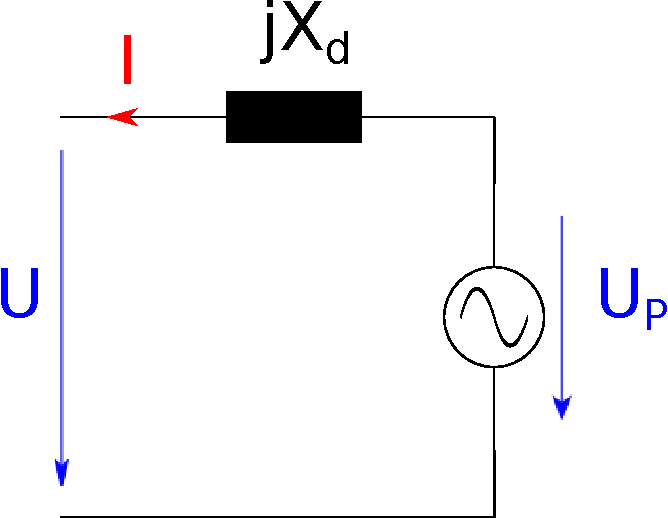
\includegraphics[scale=.4]{./img/ersatzschaltbild_synchronmaschine.pdf}
		\end{center}		
		\[X_d = \omega \cdot (L_h + L_\sigma)\]
		\[X_d \cdot I_w = U_p \sin(\vartheta_M)\]
		\[X_d = x_d \frac{U_r^2}{S_r}\]		
		übererregt: wirkt wie Kapazität, gibt induktive Blindleistung ab \\
		unterregt: wirkt wie Induktivität, nimmt induktive Blindleistung auf \\		
		Kippmoment $M_k$; Betrieb bei ca. $\frac{2}{3} M_k \Rightarrow \vartheta_M < 42^\circ$\\		
		\begin{center}
		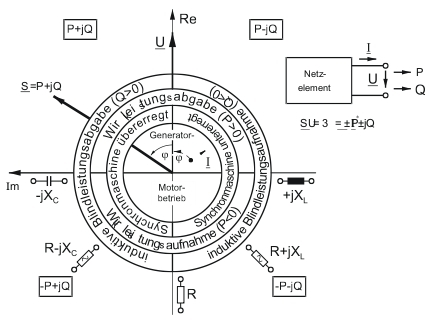
\includegraphics[scale=.75]{./img/synchronmaschine_betriebsbereiche.jpg}
		\end{center}
		
		\subsection{Asynchronmaschine}		
		\begin{center}
		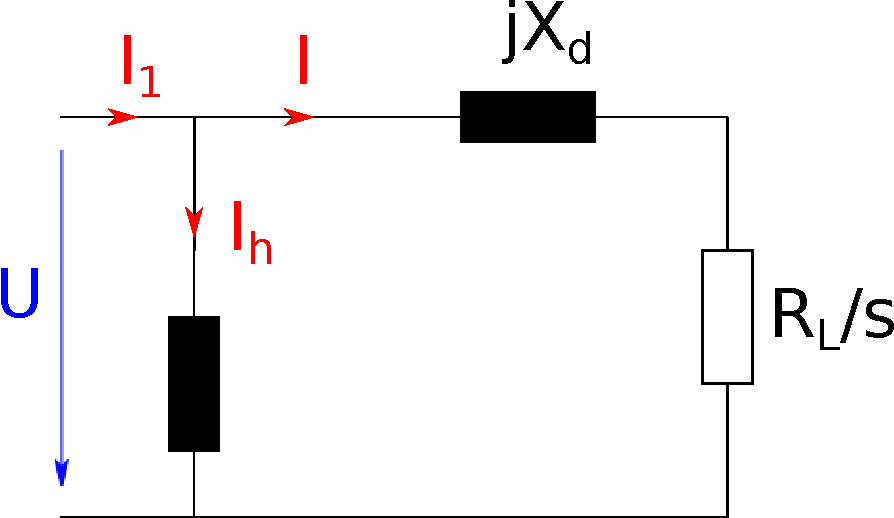
\includegraphics[scale=.4]{./img/ersatzschaltbild_asynchronmaschine.pdf}
		\end{center}		 
		\[s = \frac{n_0 - n}{n_0}\]
		\[M = \frac{3}{2 \pi n_0} \frac{I^2 R_l}{s}\]
		\[n_0 = \frac{f}{p}\]
		\[M = \frac{2 M_k}{\frac{s}{s_k} + \frac{s_k}{s}}\]
		Anlauf nur möglich falls $M_A < M_{an}$; $U$ kann nicht beliebig erhöht werden $\Ra$ Fluss wird kleiner $\Ra$ Moment wird kleiner		
		\[\eta = 1 - s\]
		\[s_k = \frac{R_L}{X_\sigma}\]
		\[M_k = \frac{3}{2 \pi n_0} \frac{U^2}{2 X_\sigma}\]		
		
	\section{Elektrische Energieübertragung}	
		\subsection{Leitungsmatrizen}		
		% einphasiges ESB für den symmetrischen Betrieb
		
		\[\begin{pmatrix} \vec U_1 \\ \vec U_2 \\ \vec U_3 \end{pmatrix} = \begin{pmatrix} \vec Z_d & \vec Z_k & \vec Z_k \\ \vec Z_k & \vec Z_d & \vec Z_k \\ \vec Z_k & \vec Z_k & \vec Z_d \end{pmatrix} \begin{pmatrix} \vec I_1 \\ \vec I_2 \\ \vec I_3 \end{pmatrix}\]
		Im symmetrischen Betrieb kann im einphasigen ESB $Z_b$ als Leitungsimpedanz eingesetzt werden:
		\[\vec Z_b = \vec Z_d - \vec Z_k\]
		
		\subsection{Leitungsbetrachtungen}
		Leitungswinkel: 
		\[\vartheta = \varphi_{u1} - \varphi_{u2}\]
		\[\vec Z_w = \sqrt{\frac{R' + j \omega L_b'}{G_b' + j \omega C_b'}}\]
		\[\vec \gamma = \sqrt{(R' + j \omega L_b')(G_b' + j \omega C_b')}\]
		\[\begin{pmatrix} \vec U_1 \\ \vec I_1 \end{pmatrix} = \begin{pmatrix} \cosh(\vec \gamma l) & \vec Z_w \sinh(\vec \gamma l) \\ \frac{1}{\vec Z_w} \sinh(\vec \gamma l) & \cosh(\vec \gamma l) \end{pmatrix} \begin{pmatrix} \vec U_2 \\ \vec I_2 \end{pmatrix}\]
		$\pi$-Ersaztschaltbild:
		\[\vec Z_l' = \vec Z_w \sinh(\vec \gamma l)\]
		\[\vec Y_q / 2 = \frac{1}{\vec Z_w} \tanh(\vec \gamma \frac{l}{2})\]

		\subsection{Vereinfachte Leitungsbetrachtung}		
		% einphasiges ESB		
		Vernachlässigung von Queradmittanzen $\Ra$ $I_{1} = I_{2}$ \\
		ohmsch induktive Last:
		\[\Delta U = R \cdot I_w + \omega L_b I_b\]
		\[\delta U = \omega L_b I_w - R I_b\]
		ohmsch kapazitive Last:
		\[\Delta U = R \cdot I_w - \omega L_b I_b\]
		\[\delta U = \omega L_b I_w + R I_b\]
		
		\[P_V = P_1 - P_2 = 3 I^2 R\]
		\[Q_V = Q_1 - Q_2 = 3 I^2 \omega L_b\]
		\[\vec U_1 = \vec U_2 + \Delta U + j \delta U\]
		falls $R << \omega L_b$ \quad $\Ra \vec U_{12} = j \omega L_b (I_w + j I_b)$
		
		\subsection{Verlustfreie Hochspannungsfernleitung}		
		% einphasiges ESB		
		\[Z_W = \sqrt{\frac{\omega L'_b}{\omega C'_b}}\]
		\[\beta = \sqrt{\omega L'_b \omega C'_b}\]
		\[\vec U_1 = \vec U_2 \cos (\beta l) + j Z_W \sin (\beta l) \vec I_2\]
		\[\vec I_1 = j \frac{\vec U_2}{Z_W} \sin (\beta l) + \vec I_2 \cos (\beta l)\]
		\[P_{nat} = \frac{U_n^2}{Z_W}\]		
		\begin{tabular}{lcc}
		 & elektrisch kurz \\
		Freileitung & $\le 200$ km \\
		Kabel & $\le 100$ km
		\end{tabular}	
			
		\begin{tabular}{lll}
		& $\vec Z_l$ & $\frac{\vec Y_q}{2}$\\[0.5em] \midrule
		el. lange Leitung & $\i Z_w \sin(\beta l)$ & $\frac{\cos(\beta l) -1}{\i Z_w \sin(\beta l)}$\\[0.5em]
		el. kurze Leitung & $\i \omega L'_b l$ & $\frac{\i \omega C'_b l}{2}$\\[0.5em]
		\end{tabular}		
		
		Bei Übertragung der natürlichen Leistung:
		\[\vec U_1 = \vec U_2 e^{j \beta l}\]
		\[\vec I_1 = \vec I_2 e^{j \beta l}\]
		
		\subsection{Blindleistungskompensation}
		\[Z_{wk} = Z_w \sqrt{\frac{1 - k_l}{1 - k_q}}\]
		\[\beta_k = \beta \sqrt{(1 - k_l)(1 - k_q)}\]		
		\[L_w' = L' (1 - k_l)\]
		\[C_w' = C' (1 - k_q)\]		
		\[\frac{P_{natk}}{P_{nat}} = \sqrt{\frac{1 - k_q}{1 - k_l}}\]
		Querkompensationsinduktivität am Ende der Leitung für ideale Kompensation im Leerlauf:
		\[X_k = \frac{Z_W \sin (\beta l)}{1 - \cos (\beta l)}\]
		Querkompensationsblindleistung am Ende der Leitung mit Spulen in Sternschaltung, ideale Kompensation:
		\[Q_2 = \frac{P_{nat}}{\sin (\beta l)} \left[ \sqrt{1 - \left( \frac{P_2}{P_{nat}} \sin (\beta l) \right)^2} - \cos (\beta l)\right] \]		
		Längskompensation, einstufig:
		\[k_l = \frac{\frac{1}{\omega C_k}}{\omega L' l}\]
		Faustformel für die Anzahl der Kondensatorbatterien: \\
		$0 < k_l \le 0,5 \Rightarrow n = 1$
		
		\begin{tabular}{c|c|c}
		& $n$ & $X_k$ \\ \hline
		$0 < k_l \le 0,5$ & 1 & $k_l \cdot 2 \cdot Z_w \cdot \sin (\beta \frac{l}{2})$ \\ \hline
		$0,5 < k_l \le 0,67$ & 2 & $k_l \cdot \frac{3}{2} \cdot Z_w \cdot \sin (\beta \frac{l}{3})$ \\ \hline
		$0,67 < k_l \le 0,75$ & 3 & $k_l \cdot \frac{4}{3} \cdot Z_w \cdot \sin (\beta \frac{l}{4})$
		\end{tabular}
		
		\subsection{Leitungsbeläge Freileitung}
		Angaben:
		\[\underbrace{4}_{Anzahl\ Leiter} \cdot \underbrace{21,7}_{Radius\ Leiter} / \underbrace{400}_{Abstand\ Leiter} mm\]
		$r_T$ ... Radius des Leiterbündels \\
		$r_B$ ... Ersatzradius für ein Leiterbündel \\
		$D$ ... Ersatzabstand zwischen zwei Leitern \\
		$h$ ... Ersatzhöhe einer Freileitung
		\[r_b = \sqrt[n]{n \cdot r \cdot r_T^{n - 1}}\]
		\[D_{einfach} = \sqrt[3]{D_{12} \cdot D_{23} \cdot D_{31}}\]
		\[D_{doppelt} = \sqrt[3]{D_{12} \cdot D_{23} \cdot D_{31} \frac{D_{12'} \cdot D_{23'} \cdot D_{31'}}{D_{11'} \cdot D_{22'} \cdot D_{33'}}}\]
		\[h = \sqrt[3]{h_1 \cdot h_2 \cdot h_3}\]
		\[h_{eff} = h - 0,7 \cdot f_{max}\]
		\[Q_{eff} = n \cdot Q\]
		\[R'(\vartheta) = \frac{1}{\kappa_{20} Q_{eff}} \left[1 + \alpha (\vartheta/(1^\circ C) \cdot K - 20 K) \right]\]
		\[L'_b = \left( 2 \ln \frac{D}{r_B} + \frac{1}{2n} \right) \cdot 10^{-4} H/km\]
		\[C'_b = \frac{2 \pi \epsilon_0}{\ln \frac{D_{ers}}{r_B \sqrt{1 + \left(\frac{D_{ers}}{2 h_{eff}}\right)}}}\]
		falls $D_{ers} << 2h_{eff}$:
		\[C'_b = \frac{2 \pi \epsilon_0}{\ln \frac{D_{ers}}{r_B }}\]
		\[G'_b = \frac{P'_V}{U_n^2}\]
		Berechnung der Kapazität im Mitsystem $C_b$ mit Leiter-Erd-Kapazität $C_E$ und Leiter-Leiter-Kapazität $C_L$:
		\[C_b = 3 \cdot C_L + C_E\]
		
		\subsection{Leitungsbeläge Kabel}
		\[R'(\vartheta) = \frac{1}{\kappa_{20} Q} \left[1 + \alpha (\vartheta/(1^\circ C) \cdot K - 20 K) \right]\]
		\[R_{AC} = (1 + y_S) R_{DC}\]
		\[y_S = \frac{x_S^4}{192 + 0,8 x_S^4}\]
		\[x_S = \sqrt{\frac{2 \mu f k_S}{R_{DC}'}}\]
		\[k_S = \begin{cases} 1 & \text{Rundleiter} \\ 0,5 & \text{Segmentleiter ein- und mehrdrätig} \end{cases}\]
		\[L_b' = \left( 2 \ln \frac{D}{r} + \frac{1}{2} \right) \cdot 10^{-4} H/km\]
		Hohlleiter, falls $0 < \frac{r_a -r_i}{r_a} < 0,6$
		\[L'_{hohl} = L'_b (0,96 + 0,051 \frac{r_a -r_i}{r_a})\]
		Radialfeldkabel(drei einzelne Leiter mit jeweils eigenen Abschirmungen):
		\[C_b' = \frac{2 \pi \epsilon}{\ln \frac{R_a}{R_i}}\]
		Gürtelkabel (drei Leiter mit einem gemeinsamen Schirm):
		\[C_b' = \frac{2 \pi \epsilon}{ln \sqrt{\frac{3 c^2 (R_a^2 - c^2)^3}{R_i^2(R_a^6 - c^6)}}}\]
		\[G_b' = \tan \delta \omega C_b'\]
		
		\subsection{Netzeinspeisung}
		\[Z_Q = \frac{c U_{nQ}}{\sqrt{3} I''_{kQ}}\]
		\[Z_Q = c \frac{U_{nQ}^2}{S''_{kQ}}\]
		
		\subsection{Kurzschlussstromberechnung}
		\[I''_{k3} = \frac{c \frac{U_{nN}}{\sqrt 3}}{Z_{(1)}}\]
		im unvermaschten Netz mit Stromverzweigungen:
		\[i_{p,i} = \kappa_i \sqrt 2 I_{K,i}''\]
		\[i_p = \sum_i i_{p,i}\]
		\[\kappa = 1.02 + 0.98 e^{-3 \frac{R}{X}}\]
		im vermaschten Netz, Alternative 1: Berechne Kappa aus dem kleinsten $\frac{R}{X}$ aller möglichen speisenden Zweige
		\[i_p = \kappa \sqrt 2 I_K''\]
		im vermaschten Netz, Alternative 2: Berechne Kappa aus $\frac{R}{X}$ von $Z_k$; solange die Verhältnisse $\frac{R}{X}$ in allen Zweigen kleiner als $0.3$ ist kann der Faktor $1.15$ weg gelassen werden; in Niederspannungsnetzen wird $1.15 \kappa$ auf $1.8$, in Mittel- und Hochspannungsnetzen auf $2.0$ begrenzt
		\[i_p = 1.15 \kappa \sqrt 2 I_K''\]\\
		\\
		\begin{tabular}{l|c|c}
		zweipolig, ohne Erde & $I_{k2}'' = \frac{\sqrt{3}}{2} I_k''$ & $i_{p2} = \kappa \sqrt{2} I_{k2}''$ \\ \hline
		zweipolig, mit Erde & $I_{k2E}'' = \frac{\sqrt{3} c U_n}{|\vec Z_{(1)} + 2 \vec Z_{(0)}|}$ & $i_{p2E} = \kappa \sqrt{2} I_{k2E}''$ \\ \hline
		einpolig & $I_{k1}'' = \frac{\sqrt{3} c U_n}{|2 \vec Z_{(1)} + \vec Z_{(0)}|}$ & $i_{p1} = \kappa \sqrt{2} I_{k1}''$
		\end{tabular}

	\section{Hochspannungstechnik}
		\subsection{Gasdurchschlag}
		\[p = \frac{r + d}{r}\]
		$r$: Radius des stärker gekrümmten Betriebsmittels
		\[\eta = \frac{E_{mittel}}{E_{max}} = \frac{U/s}{E_{max}}\]
		\[U_i = E_{dh} \cdot s \cdot \eta\]
		\[U_s = E_s \cdot s\]
		\[U_d = \max\{U_i, U_s\}\]
		\[E_{dh,Luft} = 25 \hdots 50 \frac{kV}{cm}\]
		\begin{tabular}{l|c}
		 & $E_s / \frac{kV}{cm}$ \\ \hline
		 positive Gleichspannung & $4,5$ \\ \hline
		 negative Gleichspannung & $5 \hdots 10$ \\ \hline
		 Wechselspannung & $4,5$
		\end{tabular}
		
		Richtwerte: \\
		\[\left( \frac{E}{p}\right)_{0,Luft} = 25.9 \frac{kV}{mm MPa}\]
		\[\left( \frac{E}{p}\right)_{0,SF_6} = 89.2 \frac{kV}{mm MPa}\]
		
		\subsubsection{Ionisationskoeffizienten}
		\paragraph{Luft} \hfill \\
		\begin{tabular}{l|c}
		$\frac{E}{p} / \frac{kV}{mm MPa}$ & $\frac{\overline \alpha}{p} / \frac{1}{mm MPa}$ \\ \hline
		$< 75$ & $0.1605 \left( \frac{mm MPa}{kV} \right)^2 \left(\frac{E}{p} - \frac{21.65 kV}{mm MPa} \right)^2 - 2,873 $ \\
		$> 75$ & $16.8 \frac{mm MPa}{kV} \frac{E}{p} - 800$
		\end{tabular}
		\paragraph{SF\textsubscript{6}} \hfill \\
		\begin{tabular}{l|c}
		$\frac{E}{p} / \frac{kV}{mm MPa}$ & $\frac{\overline \alpha}{p} / \frac{1}{mm MPa}$ \\ \hline
		$< 125$ & $27.9 \frac{mm MPa}{kV} \left( \frac{E}{p} - 89.2 \frac{kV}{mm MPa} \right)$ \\
		$> 125$ & $22.4 \frac{mm MPa}{kV} \frac{E}{p} -1802$
		\end{tabular}
		
		\subsubsection{Streamer}
		Streamer-Kriterium ($K = 9.15$ für Luft, $K = 10.5$ für SF\textsubscript{6}):
		\[\int_0^{x_c} (\alpha - \eta) dx = \int_0^{x_c} \overline \alpha dx \ge K\]

		\subsection{Lichtbogen}
		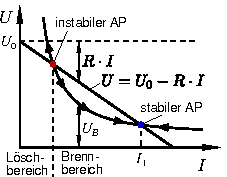
\includegraphics[scale=1.4]{./img/Lichtbogen.pdf}\\
		Ayrton-Gleichung: 
		\[U_B = U_0 - R \cdot I_B = a + bl + \frac{c+dl}{I_B}\]
		Determinante = 0 $\Rightarrow R \ra \text{max};\ U_{B} \ra \text{min}$\\
		\\
		Löschblechabstand von wenigen mm: $U_B = 20$V
		\[n \cdot U_B > U_0\]

		\subsection{Stoßspannungsgenerator (Typ B)}
		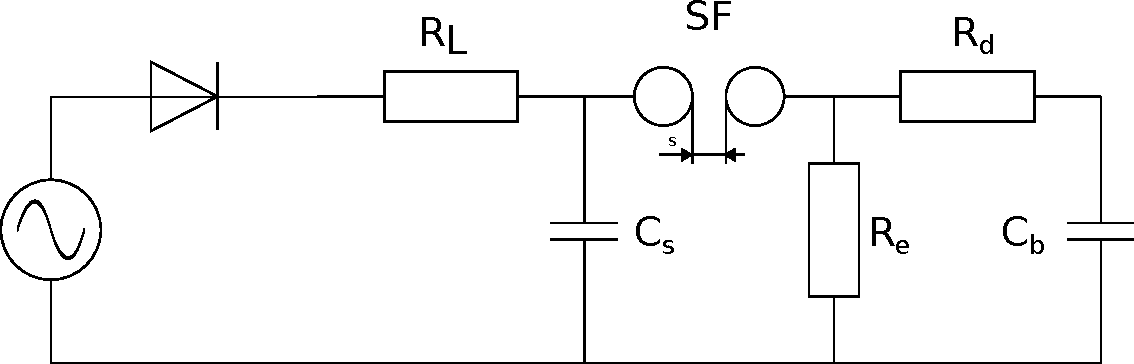
\includegraphics[scale=0.4]{./img/stossspannungsgenerator_einstufig_schaltung_b.pdf}\\
		\[u(t) = \frac{U_0}{R_d C_b} \frac{\tau_1 \tau_2}{\tau_1 - \tau_2} \left(e^{-\frac{t}{\tau_1}} - e^{-\frac{t}{\tau_2}} \right)\]
		\[\eta_{Stoß} = \frac{\hat u(t)}{U_0}\]
		\[\tau_1 \approx R_e (C_s + C_b)\]
		\[\tau_2 \approx R_d \frac{C_s C_b}{C_s + C_b}\]
		\[\eta_{Stoß} \approx \frac{C_s}{C_s + C_b}\]
		\begin{tabular}{c|c|c|c|c}
		$T_p/T_2$ & $T_1/T_2$ & $k_1$ & $k_2$ & $k_3$ \\ \hline
		& 1,2/50 & 0,733 & 2,963 & \\ \hline
		250/2500 & & 0,7924 & & 4,001
		\end{tabular} \\
		$T_1 = k_2 \tau_2$, $T_2 = k_1 \tau_1$, $T_p = k_3 \tau_2$ \\
		Mehrstufig:\\
		\[C_s = \frac{1}{n} C'_s\]
		\[U_{0,ges} = n \cdot U_0\]
		\[R_e = n R'_e\]
		\[R_d = n R'_d\]
		\[W_{Entlade} = \frac{1}{2} C_S U_0^2\]
		\[W_{Lade} = 2 \cdot W_{Entlade}\]

		\subsection{Greinacher-Kaskadenschaltung}
		\[\overline U_0 = 2 n \hat u_T\]
		\[\delta U = \frac{\overline I_g}{2 f C} \frac{n (n + 1)}{2}\]
		\[\Delta U = \frac{\overline I_g}{f C} \left( \frac{2}{3} n^3 + \frac{1}{2} n^2 - \frac{1}{6} n \right) \]
		\[\overline U = \overline U_0 - \Delta U - \delta U\]
		
		\subsection{Feldberechnung}
		\subsubsection{Finite Elemente}
		\[\varphi_i(x_i, y_i) = a_0 + a_1 x + a_2 y\]
		\[W_el = \frac{1}{2} \int_V \epsilon_0 \epsilon_r \vec E dV\]
		\[E_A = \sqrt{a_{1A}^2 + a_{2A}^2}\]
		\[W_A = \frac{1}{2} \epsilon_0 \epsilon_{r1} A l (a_{1A}^2 + a_{2A}^2)\]
		
		\subsubsection{Ersatzladungsverfahren}
		Allgemeines Potential einer Punktladung:
		\[\Phi(\vec r) = \frac{Q}{4 \pi \epsilon \vec r}\]
		rotationssymmetrische Anordnung, Abstand $z_j$ zur Spiegelebene:
		\[p_{ij} = \frac{1}{4 \pi \epsilon} \left[ \frac{1}{\sqrt{r_i^2 + (z_i - z_j)^2}} - \frac{1}{\sqrt{r_i^2 + (z_i + z_j)^2}} \right]\]
		\[\begin{pmatrix} p_{11} & \hdots & p_{1n} \\ \vdots & & \vdots \\ p_{n1} & \hdots & p_{nn} \end{pmatrix} \begin{pmatrix} Q_1 \\ \vdots \\ Q_n \end{pmatrix} = \begin{pmatrix} \varphi_1 \\ \vdots \\ \varphi_n \end{pmatrix}\]
		
		\subsubsection{Differenzenverfahren}
		Viereckformel:
		\[\varphi_\nu = \frac{1}{4}(\varphi_E + \varphi_N + \varphi_W + \varphi_S)\]
		geschichtete Dielektrika (Dielektrikum-Übergang von N nach S von $\epsilon_{r1}$ nach $\epsilon_{r2}$):
		\[\varphi_\nu = \frac{1}{4}(\varphi_W + \varphi_E + \frac{2}{\epsilon_{r1} + \epsilon_{r2}} (\epsilon_{r1} \varphi_N + \epsilon_{r2} \varphi_S))\]
		
		\subsubsection{Mehrstoffdielektrika}
		Zylindrische Durchführung mit n Dielektrika und Metallfolien an den Grenzflächen:
		\[E_\nu(r) = \frac{U}{r l_\nu \epsilon_\nu \sum_{j=1}^n \left( \frac{1}{\epsilon_j l_j} \ln\left( \frac{r_{j+1}}{r_j}\right) \right) }\]
		
		\subsubsection{Spannungsverteilung}
		$u(a) = \frac{U_x}{U}$, $a = \frac{x}{l}$, $u(0) = 0$, $u(1) = 1$
		\[u(a) = \frac{1}{C_E + C_L} \left[ C_E \frac{\sinh(\kappa a)}{\sinh(\kappa} + C_L \left( 1 - \frac{\sinh(\kappa (1 - a))}{\sinh(\kappa} \right) \right]\]
		\[C_E = n \Delta C_E\]
		\[C_L = n \Delta C_L\]
		\[C_S = \frac{1}{n} \Delta C_s\]
		\[\kappa = \sqrt{\frac{C_E + C_L}{C_S}}\]
		
		\subsubsection{Auslegung GIS} \hfill \\
		optimales Verhältnis von Leiteraußen- und Hüllenradius:
		\[r_i = \frac{r_a}{e}\]
		Abschluss mit Kugelkondensator:
		\[E(r) = U \frac{r_i r_a}{r_a - r_i} \frac{1}{r^2}\]
		Rohrkondensator:
		\[E(r) = \frac{U}{r \ln \left( \frac{r_a}{r_i}\right)}\]
		

% Ende der Spalten
\end{multicols}

% Dokumentende
% ======================================================================
\end{document}
